\section{Besoins Métier}

%
%
\subsection{Contexte}

On se situe dans le cadre d'un établissement hospitalier, une clinique, qui souhaite développer une offre médicale dédiée aux maladies des voies respiratoires.
Pour cela un nouveau pôle est construit à 50 mètres du bâtiment déjà existant de la clinique.
Nous sommes chargés de réaliser l'étude de l'architecture réseau à implanter dans ce nouveau bâtiment.

%

Ce réseau devra répondre à une certaine tolérance aux pannes puisque utilisé à des fins médicales.
Une interconnexion avec le bâtiment adjacent sera aussi nécessaire.
Dans l'architecture réseau actuelle le cœur de réseau et l'accès à Internet se trouvent dans le bâtiment adjacent.
Le déploiement de la nouvelle portion de réseau ne devra avoir aucune incidence sur le réseau déjà existant de la clinique.
Les dimensions du bâtiment sont d'environ 35 mètres de long pour 11 mètres de large.
Il est composé de 6 étages ayant chacun différents usages.
Les différences entre ces étages seront un point de départ important pour établir l'architecture réseau :
par exemple certains équipements médicaux nécessitent d'être inter-connectés, d'autres ne doivent en aucun cas être parasités pour assurer leur fonctionnement.

%

L'objectif principal est d'assurer un service performant, péren et sécurisé tant pour le personnel que pour les patients.
Le réseau d'un hôpital ne dispose pas spécialement de performances de débit minimum mais demande une stabilité, une haute disponibilité et une sécurité très importante.
Plusieurs solutions peuvent répondre à ce cahier des charges en respectant les critères suivants et les contraintes suivantes:
\begin{itemize}
\item La fiabilite ;
\item Le coût ;
\item La sécurité ;
\item La durée de mis en place.
\end{itemize}

%
    \cleardoublepage
%

\begin{figure}[!ht]
    \center
    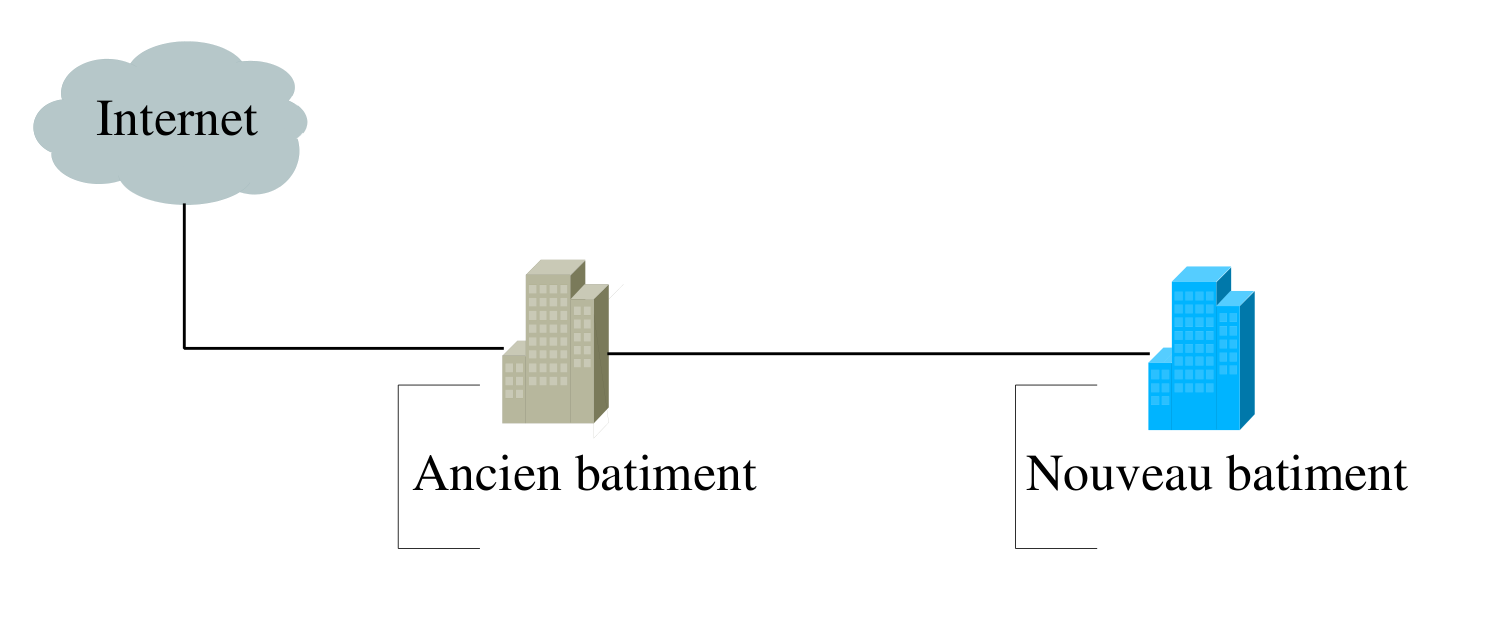
\includegraphics[width=0.8\textwidth]{./images/interco-batiment.png}
    \caption{Interconnexion du nouveau bâtiment avec l'ancien}
\end{figure}

%

L'ensemble du personnel doit pouvoir communiquer via les téléphones disponibles dans l'hôpital.
Dans l'enceinte du bâtiment, la connection d'équipements sans fil doit être rendu possible pour le personnel dans le cadre de leur travail.
L'accès à internet est fournit aux patients via une connexion sans fil.

Il n'est pas nécessaire de disposer d'une grande bande passante de façon continue.
Le personnel ne fait que de la consultation d'informations ponctuelle et les visiteurs ont un accès internet limité et non prioritaire.


%
    \cleardoublepage
%
%
\subsection{Description du bâtiment}

Il est important de savoir comment le bâtiment est conçu afin de définir les équipements et périphériques utiles aux personnels et aux patients.
Ces informations seront utiles pour déterminer l'architecture du réseau.
Dans un premier temps nous allons nous intéresser aux spécificités de chaque étage.

Le niveau -2 contient seulement un parking et les vestiaires du personnel.
Aucun accès réseau n'est nécessaire au niveau métier.
Ce niveau est aussi l'arrivée du tunnel reliant les deux bâtiments, c'est donc ici que le lien d'interconnexion des deux bâtiments est installé.
Ce lien doit monter jusqu'au rez-de-chaussée afin d'atteindre une salle dédié au infrastructure du réseau.

Le niveau -1, est l'étage le plus critique car il héberge deux blocs opératoires et quatre salles d'imageries, c'est donc ici que les équipements médicaux se situent.
Ces équipements posent certaines contraintes comme par exemple des contraintes en terme de pollution électromagnétique pour les IRM.
Les ordinateurs connectés sur ces appareils sont aussi très vulnérables : ces postes tournent sous des versions obsolètes de systèmes d'exploitation.
Ils doivent donc être isolés dans le réseau et ne pas être connectés a Internet.

Le rez-de-chaussée, appelé par la suite niveau 0, contient une salle d'accueil, une salle d'attente, trois bureaux dédiés aux personnels administratif (deux personnes par bureaux) et une salle dédiée au réseau informatique.
C'est dans cette dernière que le lien vers l'autre bâtiment sera connecté.
Cette salle contiendra donc le cœur de réseau de ce bâtiment.
Le maximum d'équipements y est aussi installer pour alléger les armoires techniques de dimensions limitées des autres étages.

Le premier étage, niveau 1, est composé de cinq bureaux de médecins, deux salles de réunions et deux laboratoire.
Cet étage est donc dédié uniquement aux personnels de la clinique.

Les trois derniers étages, les niveaux 2 à 4, sont composés des chambres des patients.
Chaque étage comporte 15 chambres ayant chacune des dimensions avoisinant les $12m^{2}$ $(4m * 3m)$.
Enfin, à chaque étage, un petit local (une armoire technique) est prévu afin de recevoir quelques équipements réseaux.


%
    \cleardoublepage
%
%
\subsection{Besoins matériels}

Il est important de connaître les technologies et périphériques nécessaires pour répondre aux besoins.
On va donc ici détailler les technologies et équipements nécessaires par étage.

\subsubsection{Niveau -2}
Aucun accès réseau n'est nécessaire à ce niveau.
Il y a l'arrivée de la fibre reliant les deux bâtiments à ce niveau.
Cette fibre est redondée et connectée à la salle réseau (le coeur du réseau) au rez-de-chaussée.

\subsubsection{Niveau -1}
Chaque bloc opératoires doit avoir au moins 2 prises Ethernet de type RJ45 afin d'y brancher les ordinateurs reliant les machines.
Un téléphone IP et un ordinateur sont installés dans chaque salle de préparation d'opération.
Dans les salles d'imageries un poste par salle et un téléphone IP sont à dispositions pour le personnel.
Les équipements médicaux sont directement reliés aux ordinateurs.

\subsubsection{Rez-de-chaussée}
C'est à ce niveau que la salle dédiée aux infrastructures réseau est située.
On y trouve une baie, sur laquelle sont raccordés les équipements tels que les serveurs, routeurs, commutateurs et le stockage des données.
L'accueil est constitué de deux téléphones IP et deux ordinateurs.
Les trois bureaux administratif ont deux téléphones et deux ordinateurs.
Des bornes WiFi sont présentes afin de fournir un accès réseau aux visiteurs.

\subsubsection{Niveau 1}
N 1 : Les bureaux des médecins contiennent chacun un téléphone IP, un ordinateur et une prise RJ45 supplémentaire.
Les imprimante peuvent être reliées en USB directement aux ordinateurs.
Les deux salles de réunions sont composées d'un téléphone IP et d'un ordinateur.
Les deux laboratoires de recherche ont un téléphone IP, deux ordinateurs et deux prises RJ45 supplémentaires.
L'étage est couvert par la WiFi.

\subsubsection{Niveaux 2 à 4}
Chaque étage contient quinze chambres pour les patients.
Les chambre disposent d'un téléphone IP. Nous ne prenons pas en compte les prises électriques ainsi que la télévision.
Le personnel présent dans l'ensemble de ces étages, bénéficient de deux postes connectés à Internet.
Un accès WiFi sera aussi disponible et bien séparé pour les patients et le personnel.
Pour la longueur du bâtiment, sur ces trente cinq mètres, deux bornes WiFi suffisent pour couvrir chaque étages.
La technologie PoE (Power Over Ethernet) sera privilégiée, permettant d'alimenter les téléphones et les bornes WiFi par le câble Ethernet.

%
%
